\section{Splay-дерево}
Splay-дерево: дерево, которое остаётся сбалансированным
в среднем и при этом не хранит никакой
дополнительной информации в вершинах;
реализация основных операций через операцию splay;
верхняя оценка $\O(\log n)$ на среднюю стоимость операций.

\subsection{Splay}
Операция splay --- перемещение
искомой вершины $x$ в корень,
делится на 3 случая:

\noindent
\begin{minipage}{\textwidth}
    Родитель $x$ --- корень,
    тогда один поворот:

    \begin{center}
        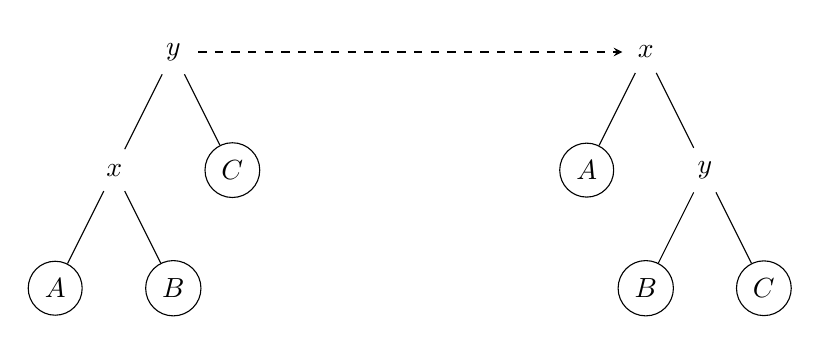
\begin{tikzpicture}[every node/.style={circle}]
            \node (x1) {$y$}
                child {
                    node {$x$}
                    child { node [draw] {$A$} }
                    child { node [draw] {$B$} }
                }
                child { node [draw] {$C$} };

            \node (x2) at (6, 0) {$x$}
                child { node [draw] {$A$} }
                child {
                    node {$y$}
                    child { node [draw] {$B$} }
                    child { node [draw] {$C$} }
                };

            \draw[->,dashed,>=stealth] (x1) -- (x2);
        \end{tikzpicture}
    \end{center}
\end{minipage}

\vspace{3em}

\noindent
\begin{minipage}{\textwidth}
    И $x$, и родитель --- левые (правые) дети,
    тогда два верхних поворота (zig-zig):

    \begin{center}
        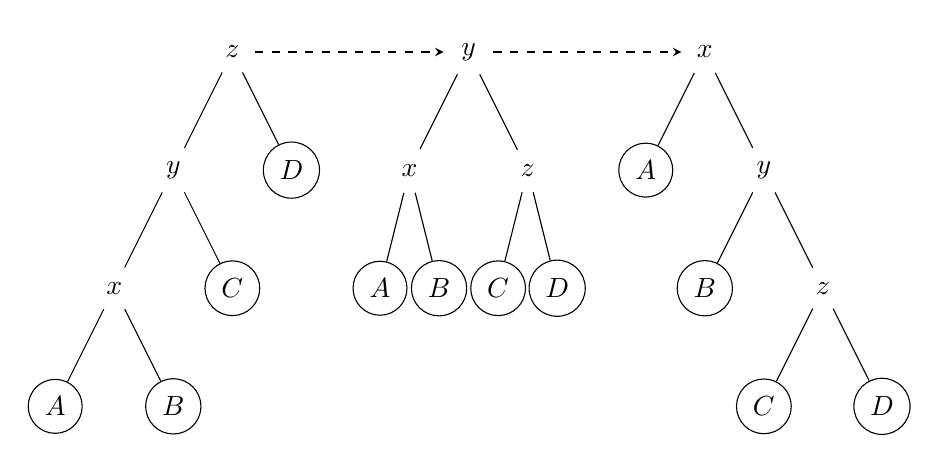
\begin{tikzpicture}[every node/.style={circle}]
            \node (x1) {$z$}
                child {
                    node {$y$}
                    child {
                        node {$x$}
                        child { node [draw] {$A$} }
                        child { node [draw] {$B$} }
                    }
                    child { node [draw] {$C$} }
                }
                child { node [draw] {$D$} };

            \node (x2) at (3, 0) {$y$}
                [level 2/.style={sibling distance=7.5mm}]
                child {
                    node {$x$}
                    child { node [draw] {$A$} }
                    child { node [draw] {$B$} }
                }
                child {
                    node {$z$}
                    child { node [draw] {$C$} }
                    child { node [draw] {$D$} }
                };

            \node (x3) at (6, 0) {$x$}
                child { node [draw] {$A$} }
                child {
                    node {$y$}
                    child { node [draw] {$B$} }
                    child {
                        node {$z$}
                        child { node [draw] {$C$} }
                        child { node [draw] {$D$} }
                    }
                };

            \draw[->,dashed,>=stealth] (x1) -- (x2);
            \draw[->,dashed,>=stealth] (x2) -- (x3);
        \end{tikzpicture}
    \end{center}
\end{minipage}

\vspace{3em}

\noindent
\begin{minipage}{\textwidth}
    $x$ --- правый ребёнок левого ребёнка (или наоборот),
    тогда сначала нижний поворот, потом верхний (zig-zag):

    \begin{center}
        \begin{tikzpicture}
            \node (x1) {$z$}
                child {
                    node {$y$}
                    child { node {$A$} }
                    child {
                        node {$x$}
                        child { node {$B$} }
                        child { node {$C$} }
                    }
                }
                child { node {$D$} };

            \node (x2) at (4, 0) {$z$}
                child {
                    node {$x$}
                    child {
                        node {$y$}
                        child { node {$A$} }
                        child { node {$B$} }
                    }
                    child { node {$C$} }
                }
                child { node {$D$} };

            \node (x3) at (8, 0) {$x$}
                [level 2/.style={sibling distance=7.5mm}]
                child {
                    node {$y$}
                    child { node {$A$} }
                    child { node {$B$} }
                }
                child {
                    node {$z$}
                    child { node {$C$} }
                    child { node {$D$} }
                };

            \draw[->,dashed,>=stealth] (x1) -- (x2);
            \draw[->,dashed,>=stealth] (x2) -- (x3);
        \end{tikzpicture}
    \end{center}
\end{minipage}

После каждой операции поиска (find) выполняется splay.

Разделение дерева (split) --- find, splay,
дальше удаляем одно из рёбер из корня и возвращаем
деревья.

Слияние двух деревьев (merge),
если в одном все элементы меньше другого:
splay от самого большого элемента меньшего дерева,
он оказывается в корне, правого ребёнка у него нет,
подвешиваем к нему второе дерево.

Добавление элемента (add):
разделяем дерево по значению элемента,
затем подвешиваем оба поддерева к новой вершине.

\begin{definition}
    Ранг вершины $x$
    --- это $r(x) = \log_2 C(x)$,
    где $C(x)$ --- количество вершин в поддереве с корнем $x$.
\end{definition}

Будем считать сумму рангов вершин как

\begin{theorem}
    Амортизированное время операции splay
    на дереве с корнем $t$ и искомой вершиной $x$
    --- $T \le 3r(t) - 3r(x) + 1$.
\end{theorem}
\begin{proof}
    Пусть $r'(x)$ --- ранг после операции,
    $y$ --- предок $x$, а $z$ --- предок $y$ (если есть).

    \paragraph{zig}
    Меняются ранги двух вершин,
    \begin{gather*}
        T = 1 + r'(x) + r'(y) - r(x) - r(y) \\
        r'(y) < r(y) \Rightarrow T \le 1 + r'(x) - r(x) = \\
        = 1 + r(y) - r(x) = 1 + r(t) - r(x) \le \\
        \le 1 + 3 r(t) - 3 r(x)
    \end{gather*}

    \paragraph{zig-zig}
    Меняются ранги $x$, $y$, $z$.
    \begin{gather*}
        T = 2 + r'(x) + r'(y) + r'(z) - r(x) - r(y) - r(z) = \\
        = 2 + r'(y) + r'(z) - r(x) - r(y) \le \\
        \le 2 + r'(y) + r'(z) - 2 r(x) \le \\
        \le 2 + r'(x) + r'(z) - 2 r(x)
    \end{gather*}

    \begin{gather*}
        (r(x) - r'(x)) + (r'(z) - r'(x)) = \\
        = \log_2 \frac{C(x)}{C'(x)} + \log_2 \frac{C'(z)}{C'(x)} = \\
        = \log_2 \frac{1 + |A| + |B|}{3 + |A| + |B| + |C| + |D|}
        + \log_2 \frac{1 + |C| + |D|}{3 + |A| + |B| + |C| + |D|}
    \end{gather*}

    Сумма выражений под логарифмами не превосходит 1.
    \[
        4ab = (a + b)^2 - (a - b)^2 \le (a + b)^2
    \]
    Поэтому произведение выражений под логарифмами
    не превосходит $1/4$, следовательно,
    \begin{gather*}
        \log_2 \frac{1 + |A| + |B|}{3 + |A| + |B| + |C| + |D|}
        + \log_2 \frac{1 + |C| + |D|}{3 + |A| + |B| + |C| + |D|} = \\
        = \log_2 \parens{
            \frac{1 + |A| + |B|}{3 + |A| + |B| + |C| + |D|} \cdot
            \frac{1 + |C| + |D|}{3 + |A| + |B| + |C| + |D|}} \le \\
        \le \log_2 \frac{1}{4} \le -2
    \end{gather*}

    \begin{gather*}
        T \le 2 + r'(x) + r'(z) - 2r(x) = \\
        = 3 (r'(x) - r(x)) - 3 (r'(x) - r(x)) + 2 + r'(x) + r'(z) - 2r(x) = \\
        = 3 (r'(x) - r(x)) + 2 - 2 r'(x) + r(x) + r'(z) \le \\
        \le 3 (r'(x) - r(x)) + 2 + (-2) = \\
        = 3 (r'(x) - r(x)) \le 1 + 3 r(t) - 3 r(x)
    \end{gather*}

    \paragraph{zig-zag}
    Меняются ранги $x$, $y$, $z$.
    \begin{gather*}
        T = 2 + r'(x) + r'(y) + r'(z) - r(x) - r(y) - r(z) = \\
        = 2 + r'(y) + r'(z) - r(x) - r(y) \le \\
        \le 2 + r'(y) + r'(z) - 2 r(x)
    \end{gather*}

    Аналогично,
    \begin{gather*}
        (r'(y) + r'(z) - 2 r(x)) - 2 (r'(x) - r(x)) = \\
        = r'(y) + r'(z) - 2 r'(x) = \\
        = \log_2 (1 + |A| + |B|) + \log_2 (1 + |C| + |D|)
        - 2 \log_2 (3 + |A| + |B| + |C| + |D|) = \\
        = \log_2 \frac{1 + |A| + |B|}{3 + |A| + |B| + |C| + |D|}
        + \log_2 \frac{1 + |C| + |D|}{3 + |A| + |B| + |C| + |D|} \le \\
        \le \log_2 \frac{1}{4} = -2
    \end{gather*}

    Поэтому
    \begin{gather*}
        T \le 2 + r'(y) + r'(z) - 2 r(x) = \\
        = 2 + r'(y) + r'(z) - 2 (r'(x) - r(x)) + 2 (r'(x) - r(x)) \le \\
        \le 2 + (-2) + 2 r'(x) - 2 r(x) = \\
        = 2 r'(x) - 2 r(x) \le 1 + 3 r'(x) - 3 r(x)
    \end{gather*}

    Таким образом, во всех трёх случаях
    $T \le 1 + 3 r(t) - 3 r(x)$.
\end{proof}

Следовательно, суммарное амортизированное время операции splay
\[ T \le 1 + 3 \log_2 n - 3 \log_2 C(x) \in \O(\log n) \]
